\begin{itemize}
	\item Both value and direction are conserved.
	\item Units of angular momentum are $kg \cdot \frac{m^2}{s} = J \cdot s$.
\end{itemize}

\paragraph{Torque} $\vec{N} = \vec{r} \times \vec{F}$.

Units of torque are $N \cdot m$.

\begin{center}
	\includegraphics[width=0.5\linewidth]{./lect14/pic1.png}
\end{center}

$$\frac{d\vec{J}}{dt} = \frac{d}{dt}\left(\vec{r} \times \vec{p}\right) = \underbrace{\frac{d\vec{r}}{dt} \times \vec{p}}_{0} + \underbrace{\vec{r} \times \frac{d\vec{p}}{dt}}_{\vec{N}}=\vec{N}$$

\paragraph{Central force} $\vec{F} =  F \hat{r}$. No torque.

\subsection{Multi-particle systems}
\begin{center}
	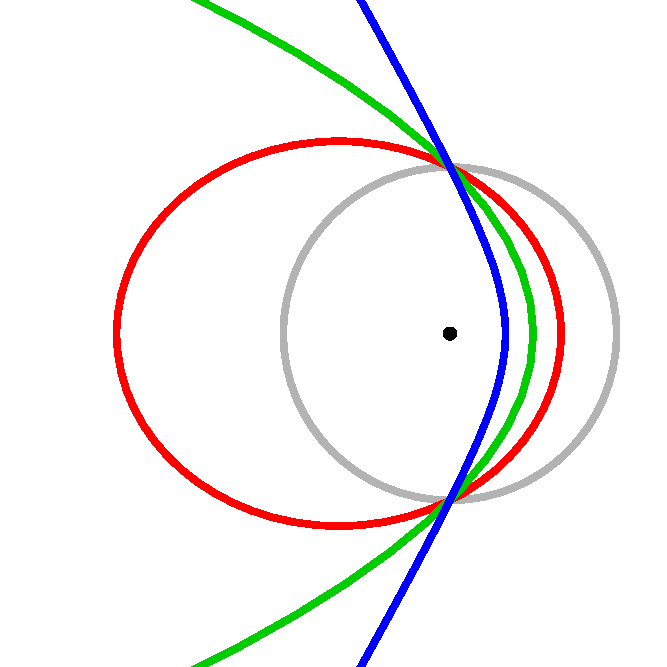
\includegraphics[width=0.8\linewidth]{./lect14/pic2.png}
\end{center}


$\vec{N}_{i\:on\:j} = \vec{r}_j \times \vec{F}_{i\:on\:j} = \vec{r}_{\perp} \times \vec{F}_{i\:on\:j}  = - \vec{r}_{\perp} \times \vec{F}_{j\:on\:i} = -\vec{r}_i  \times \vec{F}_{j\:on\:i}  = -\vec{N}_{j\:on\:i}$

Internal torques cancel each other. To calculate change in angular momentum we need to consider only external forces.

$$\vec{N} = \sum_{\parbox{1cm}{\scriptsize \centering all masses in system}} \vec{r}_i \times \vec{F}_{i\: ext}$$

A torque is around of some point so it depends on choice of origin.

\paragraph{Example} Constant gravitational force: $\vec{g} = const$. 
Total torque is $$\vec{N}_0 = \sum \vec{r}_i \times \left( m_i \vec{g} \right) \stackrel{\vec{g} = const}{=} \sum \left( \vec{r}_i m_i \right) \times \vec{g}$$

Substitute $\vec{r}_i = \vec{R}_{cm} + \vec{r}_{icm}$  

$$\vec{N}_0 = \left[ \sum \left( \vec{R}_{cm} + \vec{r}_{icm} \right)m_i  \right] \times \vec{g} = \left( \vec{R}_{cm} \sum m_i  \right) \times \vec{g} + \underbrace{\left( \sum  \vec{r}_{icm} m_i  \right) \times \vec{g}}_{0} = \left(\vec{R}_{cm} M \right) \times \vec{g} $$

In constant gravity field torque is equals to torque on point mass in center of mass: $\vec{N}_0 = \left( \vec{R}_{cm} M_{total}\right) \times \vec{g}$. Torque around center of mass is 0.
\paragraph{Non-costant gravity field} Torque around center of mass isn't 0. Moon-Earth system:

\begin{center}
	\includegraphics[width=\linewidth]{./lect14/pic3.png}
\end{center}

The torque against Earth rotation is more than torque in direction of rotation, meaning angular momentum decreases and the Earth rotation slows. Since angular momentum is conserved, Moon is drifting away from Earth.

\paragraph{Angular momentum of the body} 

\begin{align*}
\vec{J} \sum_{i=1}^{N} m_i \vec{r}_i \times \vec{v}_i = \sum m_i \left( \vec{r}_i - \vec{R}_{cm} \right) \times \vec{v}_i + \sum \vec{R}_{cm} \times \left( m_i \times \vec{v}_i \right) = \\ = \sum \vec{r}_{icm} \times \left( m_i \vec{v}_i \right) + \vec{R}_{cm} \times \sum m_i \vec{v}_i = \vec{J}_{cm} + \vec{R}_{cm} \times \vec{p}
\end{align*}

$$\vec{J}_{cm} =\vec{I}_{cm} \vec{\omega}$$
where $I$ is moment of inertia and $\omega$ is angular velocity.

\paragraph{Example} Movement of planets around Sun.
\begin{center}
	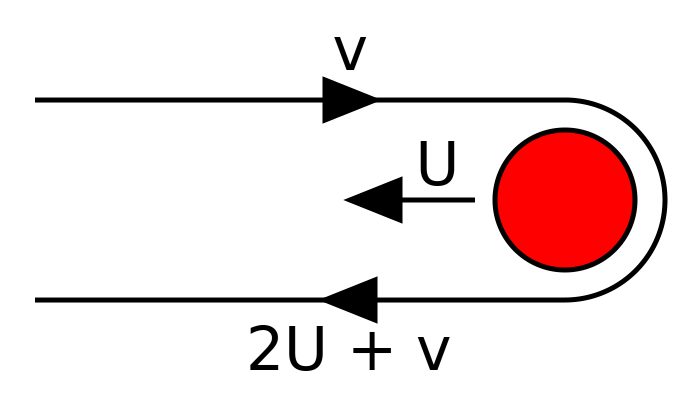
\includegraphics[width=\linewidth]{./lect14/pic4.png}
\end{center}

Area of triangle is $\vec{S} = \frac{1}{2} \vec{r} \times \Delta \vec{r}$. Derive the area:

$$\frac{d\vec{S}}{dt} = \frac{1}{2} \frac{\vec{r}  \times \Delta \vec{r}}{\Delta t} = \frac{1}{2} \vec{r} \times \frac{\Delta \vec{r}}{\Delta t} = \frac{1}{2} \vec{r} \vec{v} = \frac{1}{2} \frac{\vec{r} \times \left( m \vec{v} \right)}{m} = \frac{\vec{r} \times \vec{p}}{2m} = \frac{\vec{J}}{2m}$$

We acquired that $\frac{d\vec{S}}{dt} = const$, meaning in same time $dt$ a planet covers same area, which is second law of Kepler.
\paragraph{Example} Angular acceleration at the process of crash.

$J = mvr =  mv_0r_0 =const$ (there is only central force). Then $v = v_0 \frac{r_0}{r}= \frac{J}{mr}$. If r decreases, then v increases, since $\vec{J}$ is constant and kinetic energy increases too.

$$E_k = \frac{1}{2}mv^2 = \frac{1}{2}m \left( \frac{J}{mr} \right)^2$$
$$E_k = \frac{J^2}{2mr^2}$$

Change in kinetic energy is caused by force directed inside and its work is:

$$U_c = - \int_{\infty}^{r} F_{centrifugal} dr = - \int_{\infty}^{r} \frac{mv^2}{r} dr $$

We substitute $v  =\frac{J}{mr}$, i.e. $F_{centrifugal} = \frac{J^2}{mr^3}$. Then the work is:

$$U_c = - \int_{\infty}^{r} \frac{J^2}{mr^3} dr = -\left[ \frac{J^2}{2mr^2} \right]_{\infty}^{r} =- \frac{J^2}{2mr^2}$$

which is equal to change in kinetic energy. \textbf{Note:} this works only when angular momentum is constant.

